\documentclass[11pt,a4paper]{article}
\usepackage[margin=25mm]{geometry}
\usepackage{amsmath,amssymb,amsthm}
\usepackage{hyperref}
\usepackage{tikz}
\usetikzlibrary{arrows.meta}
\hypersetup{colorlinks=true,urlcolor=blue,linkcolor=blue}
\newtheorem{proposition}{Proposition}
\newcommand{\diag}{\operatorname{diag}}
\newcommand{\Id}{I}
\title{A six-node counterexample to generic local implying\texorpdfstring{\\}{ }generic global network identifiability}
\author{Research note prepared with Codex}
\date{8 October 2026}
\begin{document}
\maketitle

\begin{abstract}
We construct a directed network with six nodes, nine independent unknown
edge transfer functions, three excited nodes and three measured nodes.
Its observation map $F(G)=C(I-G)^{-1}B$ has generic fiber cardinality two
and a generically nonsingular Jacobian. Thus generic local identifiability
does not imply generic global identifiability under the well-posedness
assumptions in Legat and Hendrickx (2020). No unknown input or measurement
matrices, repeated parameter constraints, known nonzero edges, or self-loops
are used. A stronger admissibility condition $\rho(G)<1$, introduced in
later work, excludes the alternative branch in this example; the result
does not refute that more restricted formulation.
\end{abstract}

\paragraph{Model and scope.}
The original question concerns $w=Gw+Br$, $y=Cw$, with fixed node selection
matrices $B,C$ and independently unknown entries of $G$ on a prescribed
graph. The 2020 paper assumes that $I-G$ is invertible and studies the map
at a fixed complex frequency \cite{LH20}. In the notation of the supplied
paper, $P=I-G$, $Q=B$, $R=C$, $S=0$.
All generic statements below mean outside a proper algebraic subset of
the nine-dimensional parameter space. The same rational identities hold
over $\mathbb C(q)$.

Set
\[
 A=\begin{pmatrix}0&0&a_3\\a_1&0&0\\0&a_2&0\end{pmatrix},\qquad
 D=\begin{pmatrix}0&d_1&0\\0&0&d_2\\d_3&0&0\end{pmatrix},\qquad
 X=\diag(x_1,x_2,x_3),
\]
and define
\begin{equation}\label{eq:model}
 G=\begin{pmatrix}A&0\\X&D\end{pmatrix},\qquad
 B=\begin{pmatrix}I_3\\0\end{pmatrix},\qquad
 C=\begin{pmatrix}0&I_3\end{pmatrix}.
\end{equation}
The nine symbols $a_i,d_i,x_i$ are independent unknowns.
Nodes $1,2,3$ are excited and nodes $4,5,6$ are measured.
The two directed cycles run in opposite directions, and three edges join
corresponding nodes from the excited cycle to the measured cycle.

\begin{center}
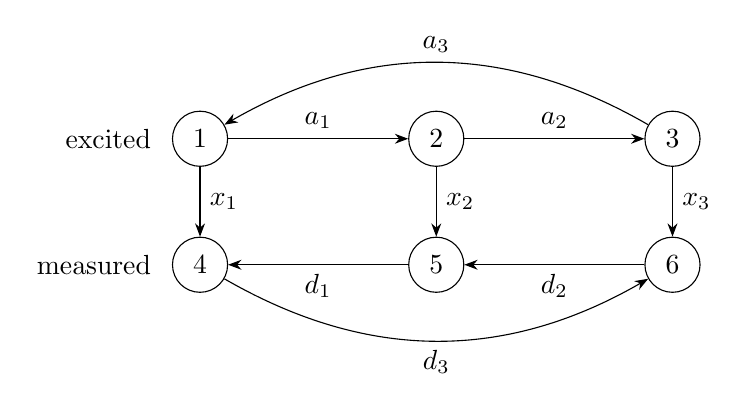
\begin{tikzpicture}[>=Stealth,vertex/.style={circle,draw,minimum size=7mm},scale=1]
\node[vertex] (1) at (0,1.6) {1};
\node[vertex] (2) at (3,1.6) {2};
\node[vertex] (3) at (6,1.6) {3};
\node[vertex] (4) at (0,0) {4};
\node[vertex] (5) at (3,0) {5};
\node[vertex] (6) at (6,0) {6};
\draw[->] (1) -- node[above] {$a_1$} (2);
\draw[->] (2) -- node[above] {$a_2$} (3);
\draw[->] (3) to[bend right=30] node[above] {$a_3$} (1);
\draw[->] (5) -- node[below] {$d_1$} (4);
\draw[->] (6) -- node[below] {$d_2$} (5);
\draw[->] (4) to[bend right=30] node[below] {$d_3$} (6);
\draw[->] (1) -- node[right] {$x_1$} (4);
\draw[->] (2) -- node[right] {$x_2$} (5);
\draw[->] (3) -- node[right] {$x_3$} (6);
\node[anchor=east] at (-0.5,1.6) {excited};
\node[anchor=east] at (-0.5,0) {measured};
\end{tikzpicture}
\end{center}

Write $\alpha=a_1a_2a_3$, $\delta=d_1d_2d_3$. Then
\[
 \det(I_6-G)=(1-\alpha)(1-\delta),\qquad
 F=(I_3-D)^{-1}X(I_3-A)^{-1}.
\]
On the generic set $x_1x_2x_3\ne0$, $F$ is invertible. Its inverse is the
particularly simple matrix
\begin{equation}\label{eq:K}
 K=F^{-1}=(I_3-A)X^{-1}(I_3-D)
 =\begin{pmatrix}
 x_1^{-1}+a_3d_3x_3^{-1}&-d_1x_1^{-1}&-a_3x_3^{-1}\\
 -a_1x_1^{-1}&x_2^{-1}+a_1d_1x_1^{-1}&-d_2x_2^{-1}\\
 -d_3x_3^{-1}&-a_2x_2^{-1}&x_3^{-1}+a_2d_2x_2^{-1}
 \end{pmatrix}.
\end{equation}

\begin{proposition}\label{prop:main}
The network structure \eqref{eq:model} is generically locally identifiable
and generically two-to-one under $G\mapsto C(I_6-G)^{-1}B$.
\end{proposition}

\begin{proof}
Introduce the invertible rational change of coordinates
\[
 u_i=a_i/x_i,\qquad v_i=d_i/x_i,\qquad z_i=1/x_i.
\]
The six off-diagonal entries of $K$ determine $u_i,v_i$ directly. Its
diagonal entries $e_i=K_{ii}$ satisfy, with indices modulo three,
\begin{equation}\label{eq:diag}
 e_i=z_i+\frac{u_{i-1}v_{i-1}}{z_{i-1}}.
\end{equation}
For fixed $u,v$, the Jacobian with respect to $z$ is
\[
 J_z=\begin{pmatrix}
 1&0&-u_3v_3/z_3^2\\
 -u_1v_1/z_1^2&1&0\\
 0&-u_2v_2/z_2^2&1
 \end{pmatrix},\qquad
 \det J_z=1-\frac{\prod_i u_iv_i}{\prod_i z_i^2}=1-\alpha\delta.
\]
Thus the full nine-dimensional observation map has Jacobian rank nine
generically. Inverting $F$ and changing parameter coordinates preserve this
rank on their domains. This proves generic local identifiability.

To prove the fiber cardinality, set $b_i=u_iv_i$. From \eqref{eq:diag},
\[
 z_2=e_2-\frac{b_1}{z_1},\qquad
 z_3=e_3-\frac{b_2}{z_2},\qquad
 z_1=e_1-\frac{b_3}{z_3}.
\]
The last equation is a fixed-point equation for a composition of three
M\"obius transformations. Clearing its denominators gives
\begin{align}\label{eq:quad}
 0={}&(b_2-e_2e_3)z_1^2\\
 &+(b_1e_3-b_2e_1-b_3e_2+e_1e_2e_3)z_1
   +b_1b_3-b_1e_1e_3.\notag
\end{align}
Generically this is a nonzero quadratic, so there are at most two
admissible solutions; $z_2,z_3$ and then $a,d,x$ are determined by $z_1$.
Zero values of $x_i$ cannot give additional solutions, because the observed
$F$ is invertible.

We now explicitly exhibit the second solution and check admissibility.
Define cyclically
\begin{equation}\label{eq:involution}
 k_i=a_id_i\frac{x_{i+1}}{x_i},\qquad
 h_i=1+k_i+k_ik_{i+1},\qquad
 r_i=\frac{k_ih_{i+1}}{h_i},\qquad
 (a_i',d_i',x_i')=\frac{1}{r_i}(a_i,d_i,x_i).
\end{equation}
These rational expressions are defined and nonzero generically.
Let $L=k_1k_2k_3=\alpha\delta$. Direct calculation gives
\[
 r_i-1=\frac{L-1}{h_i},\qquad
 r_i+\frac{k_{i-1}}{r_{i-1}}=1+k_{i-1},\qquad
 \prod_i r_i=L.
\]
The transformation leaves $u_i,v_i$ unchanged and sends $z_i$ to
$z_i'=r_iz_i$. The second identity above proves \eqref{eq:diag} is
unchanged. Therefore $K'=K$ and $F'=F$. When $L\ne1$, the first identity
shows that the two networks are distinct. Furthermore,
\[
 \alpha'=\prod_i a_i'=\frac1\delta,\qquad
 \delta'=\prod_i d_i'=\frac1\alpha,
\]
so
\[
 \det(I_6-G')=(1-1/\delta)(1-1/\alpha)\ne0
\]
whenever $\alpha\delta\ne0$ and the original network is well-posed.
The two solutions exist on a nonempty Zariski open set, and the quadratic
bound proves they exhaust the generic fiber. The Jacobian at the second
point is also nonsingular since $\alpha'\delta'=1/(\alpha\delta)\ne1$.
\end{proof}

\paragraph{A small exact numerical example.}
Let
\[
 U=\begin{pmatrix}0&0&1\\1&0&0\\0&1&0\end{pmatrix}.
\]
The following two networks have the same zero pattern:
\[
 G_1=\begin{pmatrix}\frac12U&0\\I_3&\frac13U^T\end{pmatrix},\qquad
 G_2=\begin{pmatrix}3U&0\\6I_3&2U^T\end{pmatrix}.
\]
They satisfy
\[
 C(I_6-G_1)^{-1}B=C(I_6-G_2)^{-1}B
 =\frac1{91}\begin{pmatrix}129&69&75\\75&129&69\\69&75&129\end{pmatrix},
\]
and
\[
 \det(I_6-G_1)=\frac{91}{108},\qquad \det(I_6-G_2)=182.
\]
Their equality is immediate from
\[
 F^{-1}=\frac76I_3-\frac12U-\frac13U^T,
\]
using $UU^T=I_3$. The numerical coincidences within groups of three edges
are only a convenient specialization. Proposition~\ref{prop:main} treats
all nine edges independently and proves generic ambiguity; the phenomenon
does not depend on those coincidences. The verification script also checks
a rational example with nine distinct edge values.

\paragraph{Dynamic stability versus a spectral-radius restriction.}
Both numerical examples above are proper, causal, stable constant transfer
matrices. Their internal closed-loop transfer matrices are also constant
and well-posed, hence stable in the usual input-output sense. There is no
state recursion $w_{t+1}=Gw_t$ here: the node relation is $w_t=Gw_t+Br_t$.

A nonconstant stable rational specialization is also available. Let
\[
 a(q)=\frac{q}{2(q+1/4)},\qquad
 d(q)=\frac{q}{3(q+1/5)},\qquad
 A=a(q)U,\quad D=d(q)U^T,\quad X=I_3.
\]
The companion network has
\[
 A'=d(q)^{-1}U,\qquad D'=a(q)^{-1}U^T,\qquad
 X'=[a(q)d(q)]^{-1}I_3.
\]
All entries are proper and stable. Original closed-loop cycle poles solve
$a(q)^3=1$ or $d(q)^3=1$. For a cube root of unity $\omega$, the respective
solutions have magnitudes at most
\[
 \left|\frac{2\omega(1/4)}{1-2\omega}\right|\le\frac12,
 \qquad
 \left|\frac{3\omega(1/5)}{1-3\omega}\right|\le\frac3{10}.
\]
The alternative diagonal closed-loop blocks have the same two sets of
cycle poles, exchanged; the off-diagonal block equals the original $F$.
Thus both complete networks have stable proper internal closed-loop
transfer matrices, as well as stable proper edge transfer functions.

Nevertheless, if the admissible set is additionally restricted by
$\rho(G)<1$ at the frequency under consideration, this counterexample does
not apply. Indeed, the block triangular structure gives
\[
 \rho(G)=\max\{|\alpha|^{1/3},|\delta|^{1/3}\}.
\]
If $|\alpha|,|\delta|<1$, the alternative has $\alpha'=1/\delta$ and
$\delta'=1/\alpha$, and violates that restriction. The 2024 manuscript
explicitly adds a spectral-radius assumption \cite{LH24}; it should not
be conflated with ordinary stability of rational transfer matrices. A
version imposing strictly proper edges likewise requires separate analysis.

\paragraph{Context and verification.}
The 2020 reference poses the local-to-global question in Section II and
its conclusion \cite{LH20}. Section 12.2 of Legat's 2025 thesis still
discusses it as open and reports a search with up to five unknown edges
under stated exclusions \cite{L25}. The present construction has nine.
No claim is made here about minimality or priority in the literature.

The accompanying \texttt{verify\_counterexample.py} uses exact SymPy
arithmetic to verify the rational identity $K'=K$ in nine independent
symbols, the Jacobian determinant, the quadratic fiber equation, and two
rational numerical pairs. It independently constructs the full $6\times6$
resolvents and $9\times9$ observation Jacobians at both points of each pair.
Results are recorded in \texttt{verification\_results.json}.

\begin{thebibliography}{9}
\bibitem{LH20}
A. Legat and J. M. Hendrickx,
``Local Network Identifiability with Partial Excitation and Measurement,''
\emph{59th IEEE Conference on Decision and Control}, 2020, pp. 4342--4347.
\href{https://perso.uclouvain.be/julien.hendrickx/availablepublications/LH2020_CDC.pdf}{Author's PDF}.

\bibitem{LH24}
A. Legat and J. M. Hendrickx,
``Identifiability in Networked Systems: Algebraic and Combinatorial
Conditions,'' manuscript listed by the author as submitted in August 2024.
\href{https://perso.uclouvain.be/antoine.legat/_static/TAC24.pdf}{Author's PDF}.

\bibitem{L25}
A. Legat, \emph{Generic local identifiability in dynamical networks:
from algebraic characterization to algorithms for signal selection},
Ph.D. thesis, UCLouvain, 2025, Section 12.2, pp. 162--164.
\href{https://hdl.handle.net/2078.5/256546}{Repository record}.
\end{thebibliography}
\end{document}
